\documentclass[1p]{elsarticle_modified}
%\bibliographystyle{elsarticle-num}

%\usepackage[colorlinks]{hyperref}
%\usepackage{abbrmath_seonhwa} %\Abb, \Ascr, \Acal ,\Abf, \Afrak
\usepackage{amsfonts}
\usepackage{amssymb}
\usepackage{amsmath}
\usepackage{amsthm}
\usepackage{scalefnt}
\usepackage{amsbsy}
\usepackage{kotex}
\usepackage{caption}
\usepackage{subfig}
\usepackage{color}
\usepackage{graphicx}
\usepackage{xcolor} %% white, black, red, green, blue, cyan, magenta, yellow
\usepackage{float}
\usepackage{setspace}
\usepackage{hyperref}

\usepackage{tikz}
\usetikzlibrary{arrows}

\usepackage{multirow}
\usepackage{array} % fixed length table
\usepackage{hhline}

%%%%%%%%%%%%%%%%%%%%%
\makeatletter
\renewcommand*\env@matrix[1][\arraystretch]{%
	\edef\arraystretch{#1}%
	\hskip -\arraycolsep
	\let\@ifnextchar\new@ifnextchar
	\array{*\c@MaxMatrixCols c}}
\makeatother %https://tex.stackexchange.com/questions/14071/how-can-i-increase-the-line-spacing-in-a-matrix
%%%%%%%%%%%%%%%

\usepackage[normalem]{ulem}

\newcommand{\msout}[1]{\ifmmode\text{\sout{\ensuremath{#1}}}\else\sout{#1}\fi}
%SOURCE: \msout is \stkout macro in https://tex.stackexchange.com/questions/20609/strikeout-in-math-mode

\newcommand{\cancel}[1]{
	\ifmmode
	{\color{red}\msout{#1}}
	\else
	{\color{red}\sout{#1}}
	\fi
}

\newcommand{\add}[1]{
	{\color{blue}\uwave{#1}}
}

\newcommand{\replace}[2]{
	\ifmmode
	{\color{red}\msout{#1}}{\color{blue}\uwave{#2}}
	\else
	{\color{red}\sout{#1}}{\color{blue}\uwave{#2}}
	\fi
}

\newcommand{\Sol}{\mathcal{S}} %segment
\newcommand{\D}{D} %diagram
\newcommand{\A}{\mathcal{A}} %arc


%%%%%%%%%%%%%%%%%%%%%%%%%%%%%5 test

\def\sl{\operatorname{\textup{SL}}(2,\Cbb)}
\def\psl{\operatorname{\textup{PSL}}(2,\Cbb)}
\def\quan{\mkern 1mu \triangleright \mkern 1mu}

\theoremstyle{definition}
\newtheorem{thm}{Theorem}[section]
\newtheorem{prop}[thm]{Proposition}
\newtheorem{lem}[thm]{Lemma}
\newtheorem{ques}[thm]{Question}
\newtheorem{cor}[thm]{Corollary}
\newtheorem{defn}[thm]{Definition}
\newtheorem{exam}[thm]{Example}
\newtheorem{rmk}[thm]{Remark}
\newtheorem{alg}[thm]{Algorithm}

\newcommand{\I}{\sqrt{-1}}
\begin{document}

%\begin{frontmatter}
%
%\title{Boundary parabolic representations of knots up to 8 crossings}
%
%%% Group authors per affiliation:
%\author{Yunhi Cho} 
%\address{Department of Mathematics, University of Seoul, Seoul, Korea}
%\ead{yhcho@uos.ac.kr}
%
%
%\author{Seonhwa Kim} %\fnref{s_kim}}
%\address{Center for Geometry and Physics, Institute for Basic Science, Pohang, 37673, Korea}
%\ead{ryeona17@ibs.re.kr}
%
%\author{Hyuk Kim}
%\address{Department of Mathematical Sciences, Seoul National University, Seoul 08826, Korea}
%\ead{hyukkim@snu.ac.kr}
%
%\author{Seokbeom Yoon}
%\address{Department of Mathematical Sciences, Seoul National University, Seoul, 08826,  Korea}
%\ead{sbyoon15@snu.ac.kr}
%
%\begin{abstract}
%We find all boundary parabolic representation of knots up to 8 crossings.
%
%\end{abstract}
%\begin{keyword}
%    \MSC[2010] 57M25 
%\end{keyword}
%
%\end{frontmatter}

%\linenumbers
%\tableofcontents
%
\newcommand\colored[1]{\textcolor{white}{\rule[-0.35ex]{0.8em}{1.4ex}}\kern-0.8em\color{red} #1}%
%\newcommand\colored[1]{\textcolor{white}{ #1}\kern-2.17ex	\textcolor{white}{ #1}\kern-1.81ex	\textcolor{white}{ #1}\kern-2.15ex\color{red}#1	}

{\Large $\underline{12a_{0624}~(K12a_{0624})}$}

\setlength{\tabcolsep}{10pt}
\renewcommand{\arraystretch}{1.6}
\vspace{1cm}\begin{tabular}{m{100pt}>{\centering\arraybackslash}m{274pt}}
\multirow{5}{120pt}{
	\centering
	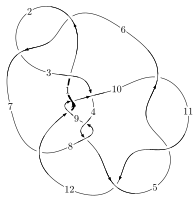
\includegraphics[width=112pt]{../../../GIT/diagram.site/Diagrams/png/1425_12a_0624.png}\\
\ \ \ A knot diagram\footnotemark}&
\allowdisplaybreaks
\textbf{Linearized knot diagam} \\
\cline{2-2}
 &
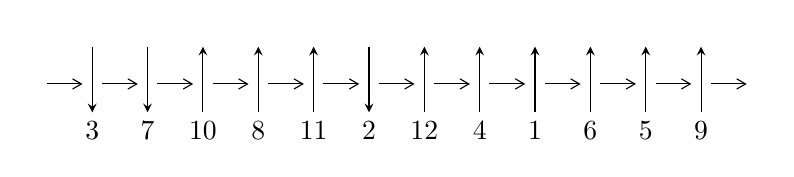
\begin{tikzpicture}[x=20pt, y=17pt]
	% nodes
	\node (C0) at (0, 0) {};
	\node (C1) at (1, 0) {};
	\node (C1U) at (1, +1) {};
	\node (C1D) at (1, -1) {3};

	\node (C2) at (2, 0) {};
	\node (C2U) at (2, +1) {};
	\node (C2D) at (2, -1) {7};

	\node (C3) at (3, 0) {};
	\node (C3U) at (3, +1) {};
	\node (C3D) at (3, -1) {10};

	\node (C4) at (4, 0) {};
	\node (C4U) at (4, +1) {};
	\node (C4D) at (4, -1) {8};

	\node (C5) at (5, 0) {};
	\node (C5U) at (5, +1) {};
	\node (C5D) at (5, -1) {11};

	\node (C6) at (6, 0) {};
	\node (C6U) at (6, +1) {};
	\node (C6D) at (6, -1) {2};

	\node (C7) at (7, 0) {};
	\node (C7U) at (7, +1) {};
	\node (C7D) at (7, -1) {12};

	\node (C8) at (8, 0) {};
	\node (C8U) at (8, +1) {};
	\node (C8D) at (8, -1) {4};

	\node (C9) at (9, 0) {};
	\node (C9U) at (9, +1) {};
	\node (C9D) at (9, -1) {1};

	\node (C10) at (10, 0) {};
	\node (C10U) at (10, +1) {};
	\node (C10D) at (10, -1) {6};

	\node (C11) at (11, 0) {};
	\node (C11U) at (11, +1) {};
	\node (C11D) at (11, -1) {5};

	\node (C12) at (12, 0) {};
	\node (C12U) at (12, +1) {};
	\node (C12D) at (12, -1) {9};
	\node (C13) at (13, 0) {};

	% arrows
	\draw[->,>={angle 60}]
	(C0) edge (C1) (C1) edge (C2) (C2) edge (C3) (C3) edge (C4) (C4) edge (C5) (C5) edge (C6) (C6) edge (C7) (C7) edge (C8) (C8) edge (C9) (C9) edge (C10) (C10) edge (C11) (C11) edge (C12) (C12) edge (C13) ;	\draw[->,>=stealth]
	(C1U) edge (C1D) (C2U) edge (C2D) (C3D) edge (C3U) (C4D) edge (C4U) (C5D) edge (C5U) (C6U) edge (C6D) (C7D) edge (C7U) (C8D) edge (C8U) (C9D) edge (C9U) (C10D) edge (C10U) (C11D) edge (C11U) (C12D) edge (C12U) ;
	\end{tikzpicture} \\
\hhline{~~} \\& 
\textbf{Solving Sequence} \\ \cline{2-2} 
 &
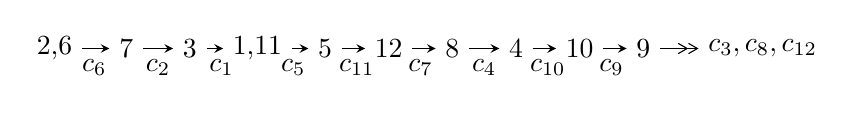
\begin{tikzpicture}[x=23pt, y=7pt]
	% node
	\node (A0) at (-1/8, 0) {2,6};
	\node (A1) at (1, 0) {7};
	\node (A2) at (2, 0) {3};
	\node (A3) at (49/16, 0) {1,11};
	\node (A4) at (33/8, 0) {5};
	\node (A5) at (41/8, 0) {12};
	\node (A6) at (49/8, 0) {8};
	\node (A7) at (57/8, 0) {4};
	\node (A8) at (65/8, 0) {10};
	\node (A9) at (73/8, 0) {9};
	\node (C1) at (1/2, -1) {$c_{6}$};
	\node (C2) at (3/2, -1) {$c_{2}$};
	\node (C3) at (5/2, -1) {$c_{1}$};
	\node (C4) at (29/8, -1) {$c_{5}$};
	\node (C5) at (37/8, -1) {$c_{11}$};
	\node (C6) at (45/8, -1) {$c_{7}$};
	\node (C7) at (53/8, -1) {$c_{4}$};
	\node (C8) at (61/8, -1) {$c_{10}$};
	\node (C9) at (69/8, -1) {$c_{9}$};
	\node (A10) at (11, 0) {$c_{3},c_{8},c_{12}$};

	% edge
	\draw[->,>=stealth]	
	(A0) edge (A1) (A1) edge (A2) (A2) edge (A3) (A3) edge (A4) (A4) edge (A5) (A5) edge (A6) (A6) edge (A7) (A7) edge (A8) (A8) edge (A9) ;
	\draw[->>,>={angle 60}]	
	(A9) edge (A10);
\end{tikzpicture} \\ 

\end{tabular} \\

\footnotetext{
The image of knot diagram is generated by the software ``\textbf{Draw programme}" developed by Andrew Bartholomew(\url{http://www.layer8.co.uk/maths/draw/index.htm\#Running-draw}), where we modified some parts for our purpose(\url{https://github.com/CATsTAILs/LinksPainter}).
}\phantom \\ \newline 
\centering \textbf{Ideals for irreducible components\footnotemark of $X_{\text{par}}$} 
 
\begin{align*}
I^u_{1}&=\langle 
-1.10901\times10^{159} u^{88}+2.62824\times10^{159} u^{87}+\cdots+1.74259\times10^{159} b-7.22250\times10^{158},\\
\phantom{I^u_{1}}&\phantom{= \langle  }1.79918\times10^{161} u^{88}-4.32262\times10^{161} u^{87}+\cdots+5.75056\times10^{160} a+7.55383\times10^{161},\;u^{89}-3 u^{88}+\cdots+25 u-3\rangle \\
\\
\end{align*}
\raggedright * 1 irreducible components of $\dim_{\mathbb{C}}=0$, with total 89 representations.\\
\footnotetext{All coefficients of polynomials are rational numbers. But the coefficients are sometimes approximated in decimal forms when there is not enough margin.}
\newpage
\renewcommand{\arraystretch}{1}
\centering \section*{I. $I^u_{1}= \langle -1.11\times10^{159} u^{88}+2.63\times10^{159} u^{87}+\cdots+1.74\times10^{159} b-7.22\times10^{158},\;1.80\times10^{161} u^{88}-4.32\times10^{161} u^{87}+\cdots+5.75\times10^{160} a+7.55\times10^{161},\;u^{89}-3 u^{88}+\cdots+25 u-3 \rangle$}
\flushleft \textbf{(i) Arc colorings}\\
\begin{tabular}{m{7pt} m{180pt} m{7pt} m{180pt} }
\flushright $a_{2}=$&$\begin{pmatrix}0\\u\end{pmatrix}$ \\
\flushright $a_{6}=$&$\begin{pmatrix}1\\0\end{pmatrix}$ \\
\flushright $a_{7}=$&$\begin{pmatrix}1\\u^2\end{pmatrix}$ \\
\flushright $a_{3}=$&$\begin{pmatrix}- u\\- u^3+u\end{pmatrix}$ \\
\flushright $a_{1}=$&$\begin{pmatrix}u^3\\u^5- u^3+u\end{pmatrix}$ \\
\flushright $a_{11}=$&$\begin{pmatrix}-3.12871 u^{88}+7.51688 u^{87}+\cdots+109.415 u-13.1358\\0.636414 u^{88}-1.50823 u^{87}+\cdots-12.0674 u+0.414469\end{pmatrix}$ \\
\flushright $a_{5}=$&$\begin{pmatrix}-0.231096 u^{88}+1.01234 u^{87}+\cdots+61.7683 u-10.7288\\2.08200 u^{88}-5.19544 u^{87}+\cdots-80.1291 u+10.3551\end{pmatrix}$ \\
\flushright $a_{12}=$&$\begin{pmatrix}0.150566 u^{88}-0.137480 u^{87}+\cdots+30.2309 u-11.3078\\0.986969 u^{88}-2.61086 u^{87}+\cdots-53.1782 u+9.36670\end{pmatrix}$ \\
\flushright $a_{8}=$&$\begin{pmatrix}2.53343 u^{88}-7.13992 u^{87}+\cdots-147.071 u+17.9792\\-1.56685 u^{88}+3.59942 u^{87}+\cdots+37.5502 u-2.31927\end{pmatrix}$ \\
\flushright $a_{4}=$&$\begin{pmatrix}-0.887414 u^{88}+1.10529 u^{87}+\cdots-9.46301 u+6.49474\\0.853902 u^{88}-2.02191 u^{87}+\cdots-14.8570 u+0.758719\end{pmatrix}$ \\
\flushright $a_{10}=$&$\begin{pmatrix}-3.76513 u^{88}+9.02512 u^{87}+\cdots+121.482 u-13.5503\\0.636414 u^{88}-1.50823 u^{87}+\cdots-12.0674 u+0.414469\end{pmatrix}$ \\
\flushright $a_{9}=$&$\begin{pmatrix}-3.82241 u^{88}+9.23994 u^{87}+\cdots+126.692 u-14.4481\\0.00747695 u^{88}+0.0854807 u^{87}+\cdots+14.4719 u-3.62999\end{pmatrix}$\\&\end{tabular}
\flushleft \textbf{(ii) Obstruction class $= -1$}\\~\\
\flushleft \textbf{(iii) Cusp Shapes $= 15.1083 u^{88}-38.1525 u^{87}+\cdots-579.178 u+94.3288$}\\~\\
\newpage\renewcommand{\arraystretch}{1}
\flushleft \textbf{(iv) u-Polynomials at the component}\newline \\
\begin{tabular}{m{50pt}|m{274pt}}
Crossings & \hspace{64pt}u-Polynomials at each crossing \\
\hline $$\begin{aligned}c_{1}\end{aligned}$$&$\begin{aligned}
&u^{89}+37 u^{88}+\cdots+229 u+9
\end{aligned}$\\
\hline $$\begin{aligned}c_{2},c_{6}\end{aligned}$$&$\begin{aligned}
&u^{89}-3 u^{88}+\cdots+25 u-3
\end{aligned}$\\
\hline $$\begin{aligned}c_{3}\end{aligned}$$&$\begin{aligned}
&1089(1089 u^{89}+13233 u^{88}+\cdots+2115 u-259)
\end{aligned}$\\
\hline $$\begin{aligned}c_{4},c_{8}\end{aligned}$$&$\begin{aligned}
&u^{89}-3 u^{88}+\cdots+25 u-3
\end{aligned}$\\
\hline $$\begin{aligned}c_{5},c_{10},c_{11}\end{aligned}$$&$\begin{aligned}
&u^{89}+u^{88}+\cdots-15 u-1
\end{aligned}$\\
\hline $$\begin{aligned}c_{7}\end{aligned}$$&$\begin{aligned}
&1089(1089 u^{89}+9075 u^{88}+\cdots+8757765 u-5706775)
\end{aligned}$\\
\hline $$\begin{aligned}c_{9},c_{12}\end{aligned}$$&$\begin{aligned}
&u^{89}- u^{88}+\cdots+17 u-1
\end{aligned}$\\
\hline
\end{tabular}\\~\\
\newpage\renewcommand{\arraystretch}{1}
\flushleft \textbf{(v) Riley Polynomials at the component}\newline \\
\begin{tabular}{m{50pt}|m{274pt}}
Crossings & \hspace{64pt}Riley Polynomials at each crossing \\
\hline $$\begin{aligned}c_{1}\end{aligned}$$&$\begin{aligned}
&y^{89}+31 y^{88}+\cdots-20963 y-81
\end{aligned}$\\
\hline $$\begin{aligned}c_{2},c_{6}\end{aligned}$$&$\begin{aligned}
&y^{89}-37 y^{88}+\cdots+229 y-9
\end{aligned}$\\
\hline $$\begin{aligned}c_{3}\end{aligned}$$&$\begin{aligned}
&1185921(1185921 y^{89}-1.88147\times10^{7} y^{88}+\cdots+2227177 y-67081)
\end{aligned}$\\
\hline $$\begin{aligned}c_{4},c_{8}\end{aligned}$$&$\begin{aligned}
&y^{89}+63 y^{88}+\cdots-59 y-9
\end{aligned}$\\
\hline $$\begin{aligned}c_{5},c_{10},c_{11}\end{aligned}$$&$\begin{aligned}
&y^{89}+91 y^{88}+\cdots+53 y-1
\end{aligned}$\\
\hline $$\begin{aligned}c_{7}\end{aligned}$$&$\begin{aligned}
&1185921(1185921 y^{89}+6.81921\times10^{7} y^{88}+\cdots+9.41156\times10^{13} y-3.25673\times10^{13})
\end{aligned}$\\
\hline $$\begin{aligned}c_{9},c_{12}\end{aligned}$$&$\begin{aligned}
&y^{89}-57 y^{88}+\cdots+53 y-1
\end{aligned}$\\
\hline
\end{tabular}\\~\\
\newpage\flushleft \textbf{(vi) Complex Volumes and Cusp Shapes}
$$\begin{array}{c|c|c}  
\text{Solutions to }I^u_{1}& \I (\text{vol} + \sqrt{-1}CS) & \text{Cusp shape}\\
 \hline 
\begin{aligned}
u &= -0.532636 + 0.845551 I \\
a &= -0.329471 + 0.111426 I \\
b &= \phantom{-}0.777464 - 0.546287 I\end{aligned}
 & \phantom{-}2.17262 - 7.81441 I & \phantom{-0.000000 } 0 \\ \hline\begin{aligned}
u &= -0.532636 - 0.845551 I \\
a &= -0.329471 - 0.111426 I \\
b &= \phantom{-}0.777464 + 0.546287 I\end{aligned}
 & \phantom{-}2.17262 + 7.81441 I & \phantom{-0.000000 } 0 \\ \hline\begin{aligned}
u &= -0.697190 + 0.706132 I \\
a &= \phantom{-}0.852079 - 1.052030 I \\
b &= -0.434773 - 0.748501 I\end{aligned}
 & \phantom{-}4.50784 + 1.34674 I & \phantom{-0.000000 } 0 \\ \hline\begin{aligned}
u &= -0.697190 - 0.706132 I \\
a &= \phantom{-}0.852079 + 1.052030 I \\
b &= -0.434773 + 0.748501 I\end{aligned}
 & \phantom{-}4.50784 - 1.34674 I & \phantom{-0.000000 } 0 \\ \hline\begin{aligned}
u &= \phantom{-}0.880484 + 0.453167 I \\
a &= \phantom{-}0.53480 + 3.00940 I \\
b &= \phantom{-}0.05012 + 1.51610 I\end{aligned}
 & -3.69992 - 1.85198 I & \phantom{-0.000000 } 0 \\ \hline\begin{aligned}
u &= \phantom{-}0.880484 - 0.453167 I \\
a &= \phantom{-}0.53480 - 3.00940 I \\
b &= \phantom{-}0.05012 - 1.51610 I\end{aligned}
 & -3.69992 + 1.85198 I & \phantom{-0.000000 } 0 \\ \hline\begin{aligned}
u &= -0.376262 + 0.908508 I \\
a &= -0.164022 - 0.085627 I \\
b &= \phantom{-}0.384148 + 0.325837 I\end{aligned}
 & \phantom{-}1.41143 + 3.84397 I & \phantom{-0.000000 } 0 \\ \hline\begin{aligned}
u &= -0.376262 - 0.908508 I \\
a &= -0.164022 + 0.085627 I \\
b &= \phantom{-}0.384148 - 0.325837 I\end{aligned}
 & \phantom{-}1.41143 - 3.84397 I & \phantom{-0.000000 } 0 \\ \hline\begin{aligned}
u &= -0.938175 + 0.401004 I \\
a &= -1.55412 + 1.82139 I \\
b &= -0.17732 + 1.87270 I\end{aligned}
 & -7.13369 + 1.50478 I & \phantom{-0.000000 } 0 \\ \hline\begin{aligned}
u &= -0.938175 - 0.401004 I \\
a &= -1.55412 - 1.82139 I \\
b &= -0.17732 - 1.87270 I\end{aligned}
 & -7.13369 - 1.50478 I & \phantom{-0.000000 } 0\\
 \hline 
 \end{array}$$\newpage$$\begin{array}{c|c|c}  
\text{Solutions to }I^u_{1}& \I (\text{vol} + \sqrt{-1}CS) & \text{Cusp shape}\\
 \hline 
\begin{aligned}
u &= \phantom{-}0.550397 + 0.885902 I \\
a &= \phantom{-}0.256430 + 0.103414 I \\
b &= -0.613597 - 0.295317 I\end{aligned}
 & \phantom{-}5.86436 + 2.38119 I & \phantom{-0.000000 } 0 \\ \hline\begin{aligned}
u &= \phantom{-}0.550397 - 0.885902 I \\
a &= \phantom{-}0.256430 - 0.103414 I \\
b &= -0.613597 + 0.295317 I\end{aligned}
 & \phantom{-}5.86436 - 2.38119 I & \phantom{-0.000000 } 0 \\ \hline\begin{aligned}
u &= -0.990809 + 0.326016 I \\
a &= -0.298513 + 0.540908 I \\
b &= -0.057054 + 0.487891 I\end{aligned}
 & -1.55145 + 1.37502 I & \phantom{-0.000000 } 0 \\ \hline\begin{aligned}
u &= -0.990809 - 0.326016 I \\
a &= -0.298513 - 0.540908 I \\
b &= -0.057054 - 0.487891 I\end{aligned}
 & -1.55145 - 1.37502 I & \phantom{-0.000000 } 0 \\ \hline\begin{aligned}
u &= \phantom{-}0.905252 + 0.530463 I \\
a &= \phantom{-}4.64241 + 0.47408 I \\
b &= -0.197180 - 0.025948 I\end{aligned}
 & -0.10358 - 2.04661 I & \phantom{-0.000000 } 0 \\ \hline\begin{aligned}
u &= \phantom{-}0.905252 - 0.530463 I \\
a &= \phantom{-}4.64241 - 0.47408 I \\
b &= -0.197180 + 0.025948 I\end{aligned}
 & -0.10358 + 2.04661 I & \phantom{-0.000000 } 0 \\ \hline\begin{aligned}
u &= -0.938122 + 0.518125 I \\
a &= -2.25920 + 1.17993 I \\
b &= \phantom{-}0.190351 + 1.357710 I\end{aligned}
 & -3.10521 + 2.76714 I & \phantom{-0.000000 } 0 \\ \hline\begin{aligned}
u &= -0.938122 - 0.518125 I \\
a &= -2.25920 - 1.17993 I \\
b &= \phantom{-}0.190351 - 1.357710 I\end{aligned}
 & -3.10521 - 2.76714 I & \phantom{-0.000000 } 0 \\ \hline\begin{aligned}
u &= -0.782728 + 0.488112 I \\
a &= \phantom{-}0.342336 + 0.940192 I \\
b &= -0.246621 - 0.071250 I\end{aligned}
 & -1.50935 + 2.07388 I & \phantom{-0.000000 } 0 \\ \hline\begin{aligned}
u &= -0.782728 - 0.488112 I \\
a &= \phantom{-}0.342336 - 0.940192 I \\
b &= -0.246621 + 0.071250 I\end{aligned}
 & -1.50935 - 2.07388 I & \phantom{-0.000000 } 0\\
 \hline 
 \end{array}$$\newpage$$\begin{array}{c|c|c}  
\text{Solutions to }I^u_{1}& \I (\text{vol} + \sqrt{-1}CS) & \text{Cusp shape}\\
 \hline 
\begin{aligned}
u &= \phantom{-}0.480693 + 0.965063 I \\
a &= -0.269333 + 0.692506 I \\
b &= \phantom{-}0.26611 + 1.53970 I\end{aligned}
 & -4.63843 + 11.63310 I & \phantom{-0.000000 } 0 \\ \hline\begin{aligned}
u &= \phantom{-}0.480693 - 0.965063 I \\
a &= -0.269333 - 0.692506 I \\
b &= \phantom{-}0.26611 - 1.53970 I\end{aligned}
 & -4.63843 - 11.63310 I & \phantom{-0.000000 } 0 \\ \hline\begin{aligned}
u &= \phantom{-}0.876714 + 0.264843 I \\
a &= \phantom{-}1.106160 + 0.454993 I \\
b &= \phantom{-}0.640905 + 1.124090 I\end{aligned}
 & -5.48696 + 0.76037 I & \phantom{-0.000000 } 0 \\ \hline\begin{aligned}
u &= \phantom{-}0.876714 - 0.264843 I \\
a &= \phantom{-}1.106160 - 0.454993 I \\
b &= \phantom{-}0.640905 - 1.124090 I\end{aligned}
 & -5.48696 - 0.76037 I & \phantom{-0.000000 } 0 \\ \hline\begin{aligned}
u &= \phantom{-}0.979855 + 0.475807 I \\
a &= \phantom{-}1.52486 + 1.95549 I \\
b &= -0.54385 + 1.67907 I\end{aligned}
 & -6.57605 - 4.05853 I & \phantom{-0.000000 } 0 \\ \hline\begin{aligned}
u &= \phantom{-}0.979855 - 0.475807 I \\
a &= \phantom{-}1.52486 - 1.95549 I \\
b &= -0.54385 - 1.67907 I\end{aligned}
 & -6.57605 + 4.05853 I & \phantom{-0.000000 } 0 \\ \hline\begin{aligned}
u &= \phantom{-}0.370514 + 0.813878 I \\
a &= \phantom{-}0.199700 - 0.361091 I \\
b &= -0.27361 - 1.53199 I\end{aligned}
 & -8.84893 + 6.12735 I & \phantom{-0.000000 } 0 \\ \hline\begin{aligned}
u &= \phantom{-}0.370514 - 0.813878 I \\
a &= \phantom{-}0.199700 + 0.361091 I \\
b &= -0.27361 + 1.53199 I\end{aligned}
 & -8.84893 - 6.12735 I & \phantom{-0.000000 } 0 \\ \hline\begin{aligned}
u &= \phantom{-}0.977486 + 0.532227 I \\
a &= \phantom{-}0.550302 + 0.974106 I \\
b &= -0.613667 + 0.315224 I\end{aligned}
 & -0.16594 - 4.11744 I & \phantom{-0.000000 } 0 \\ \hline\begin{aligned}
u &= \phantom{-}0.977486 - 0.532227 I \\
a &= \phantom{-}0.550302 - 0.974106 I \\
b &= -0.613667 - 0.315224 I\end{aligned}
 & -0.16594 + 4.11744 I & \phantom{-0.000000 } 0\\
 \hline 
 \end{array}$$\newpage$$\begin{array}{c|c|c}  
\text{Solutions to }I^u_{1}& \I (\text{vol} + \sqrt{-1}CS) & \text{Cusp shape}\\
 \hline 
\begin{aligned}
u &= \phantom{-}0.776189 + 0.801927 I \\
a &= \phantom{-}0.608392 + 0.186860 I \\
b &= -0.05077 + 1.43405 I\end{aligned}
 & -6.71130 - 2.95857 I & \phantom{-0.000000 } 0 \\ \hline\begin{aligned}
u &= \phantom{-}0.776189 - 0.801927 I \\
a &= \phantom{-}0.608392 - 0.186860 I \\
b &= -0.05077 - 1.43405 I\end{aligned}
 & -6.71130 + 2.95857 I & \phantom{-0.000000 } 0 \\ \hline\begin{aligned}
u &= \phantom{-}0.592682 + 0.654546 I \\
a &= -0.968450 - 0.900276 I \\
b &= \phantom{-}0.824689 - 0.582850 I\end{aligned}
 & \phantom{-}2.14298 + 2.52868 I & \phantom{-0.000000 } 0 \\ \hline\begin{aligned}
u &= \phantom{-}0.592682 - 0.654546 I \\
a &= -0.968450 + 0.900276 I \\
b &= \phantom{-}0.824689 + 0.582850 I\end{aligned}
 & \phantom{-}2.14298 - 2.52868 I & \phantom{-0.000000 } 0 \\ \hline\begin{aligned}
u &= -1.005190 + 0.529887 I \\
a &= -0.43796 + 1.39245 I \\
b &= \phantom{-}1.077510 + 0.640281 I\end{aligned}
 & -3.80322 + 6.41139 I & \phantom{-0.000000 } 0 \\ \hline\begin{aligned}
u &= -1.005190 - 0.529887 I \\
a &= -0.43796 - 1.39245 I \\
b &= \phantom{-}1.077510 - 0.640281 I\end{aligned}
 & -3.80322 - 6.41139 I & \phantom{-0.000000 } 0 \\ \hline\begin{aligned}
u &= \phantom{-}1.144320 + 0.059059 I \\
a &= -0.398793 + 0.894332 I \\
b &= -0.516834 + 0.697007 I\end{aligned}
 & -4.07816 - 6.32536 I & \phantom{-0.000000 } 0 \\ \hline\begin{aligned}
u &= \phantom{-}1.144320 - 0.059059 I \\
a &= -0.398793 - 0.894332 I \\
b &= -0.516834 - 0.697007 I\end{aligned}
 & -4.07816 + 6.32536 I & \phantom{-0.000000 } 0 \\ \hline\begin{aligned}
u &= -0.964012 + 0.634990 I \\
a &= \phantom{-}0.133390 - 0.352220 I \\
b &= \phantom{-}0.590169 - 0.621489 I\end{aligned}
 & \phantom{-}3.68544 + 3.81135 I & \phantom{-0.000000 } 0 \\ \hline\begin{aligned}
u &= -0.964012 - 0.634990 I \\
a &= \phantom{-}0.133390 + 0.352220 I \\
b &= \phantom{-}0.590169 + 0.621489 I\end{aligned}
 & \phantom{-}3.68544 - 3.81135 I & \phantom{-0.000000 } 0\\
 \hline 
 \end{array}$$\newpage$$\begin{array}{c|c|c}  
\text{Solutions to }I^u_{1}& \I (\text{vol} + \sqrt{-1}CS) & \text{Cusp shape}\\
 \hline 
\begin{aligned}
u &= -0.420226 + 1.077630 I \\
a &= \phantom{-}0.121883 + 0.882947 I \\
b &= -0.17022 + 1.41805 I\end{aligned}
 & \phantom{-}0.39074 - 5.12452 I & \phantom{-0.000000 } 0 \\ \hline\begin{aligned}
u &= -0.420226 - 1.077630 I \\
a &= \phantom{-}0.121883 - 0.882947 I \\
b &= -0.17022 - 1.41805 I\end{aligned}
 & \phantom{-}0.39074 + 5.12452 I & \phantom{-0.000000 } 0 \\ \hline\begin{aligned}
u &= \phantom{-}1.003450 + 0.603777 I \\
a &= -0.356046 + 0.311967 I \\
b &= -1.014410 - 0.523135 I\end{aligned}
 & \phantom{-}0.92594 - 7.45495 I & \phantom{-0.000000 } 0 \\ \hline\begin{aligned}
u &= \phantom{-}1.003450 - 0.603777 I \\
a &= -0.356046 - 0.311967 I \\
b &= -1.014410 + 0.523135 I\end{aligned}
 & \phantom{-}0.92594 + 7.45495 I & \phantom{-0.000000 } 0 \\ \hline\begin{aligned}
u &= -0.663274 + 0.482007 I \\
a &= -0.383552 - 0.098579 I \\
b &= -0.081911 + 1.222220 I\end{aligned}
 & -2.31044 + 1.39236 I & \phantom{-}6.00000 - 4.34365 I \\ \hline\begin{aligned}
u &= -0.663274 - 0.482007 I \\
a &= -0.383552 + 0.098579 I \\
b &= -0.081911 - 1.222220 I\end{aligned}
 & -2.31044 - 1.39236 I & \phantom{-}6.00000 + 4.34365 I \\ \hline\begin{aligned}
u &= -1.112340 + 0.394289 I \\
a &= -0.322205 + 0.390018 I \\
b &= -0.003884 + 0.449466 I\end{aligned}
 & -1.56596 + 1.33194 I & \phantom{-0.000000 } 0 \\ \hline\begin{aligned}
u &= -1.112340 - 0.394289 I \\
a &= -0.322205 - 0.390018 I \\
b &= -0.003884 - 0.449466 I\end{aligned}
 & -1.56596 - 1.33194 I & \phantom{-0.000000 } 0 \\ \hline\begin{aligned}
u &= -1.206400 + 0.133026 I \\
a &= \phantom{-}0.43556 - 2.50716 I \\
b &= \phantom{-}0.15758 - 1.60691 I\end{aligned}
 & -14.1434 - 3.4037 I & \phantom{-0.000000 } 0 \\ \hline\begin{aligned}
u &= -1.206400 - 0.133026 I \\
a &= \phantom{-}0.43556 + 2.50716 I \\
b &= \phantom{-}0.15758 + 1.60691 I\end{aligned}
 & -14.1434 + 3.4037 I & \phantom{-0.000000 } 0\\
 \hline 
 \end{array}$$\newpage$$\begin{array}{c|c|c}  
\text{Solutions to }I^u_{1}& \I (\text{vol} + \sqrt{-1}CS) & \text{Cusp shape}\\
 \hline 
\begin{aligned}
u &= -0.781572 + 0.064438 I \\
a &= -0.076040 - 1.012340 I \\
b &= -0.766778 + 0.017173 I\end{aligned}
 & -2.05830 - 2.27656 I & \phantom{-}1.43905 + 3.82974 I \\ \hline\begin{aligned}
u &= -0.781572 - 0.064438 I \\
a &= -0.076040 + 1.012340 I \\
b &= -0.766778 - 0.017173 I\end{aligned}
 & -2.05830 + 2.27656 I & \phantom{-}1.43905 - 3.82974 I \\ \hline\begin{aligned}
u &= \phantom{-}0.638409 + 0.407830 I \\
a &= -0.756928 - 0.235077 I \\
b &= \phantom{-}0.545634 + 0.053149 I\end{aligned}
 & \phantom{-}0.925151 - 0.025658 I & \phantom{-}11.59100 - 0.67651 I \\ \hline\begin{aligned}
u &= \phantom{-}0.638409 - 0.407830 I \\
a &= -0.756928 + 0.235077 I \\
b &= \phantom{-}0.545634 - 0.053149 I\end{aligned}
 & \phantom{-}0.925151 + 0.025658 I & \phantom{-}11.59100 + 0.67651 I \\ \hline\begin{aligned}
u &= -0.277680 + 0.700999 I \\
a &= -0.473863 - 0.710002 I \\
b &= \phantom{-}0.126131 - 1.373140 I\end{aligned}
 & -3.64108 - 2.19676 I & \phantom{-}3.44360 + 2.93374 I \\ \hline\begin{aligned}
u &= -0.277680 - 0.700999 I \\
a &= -0.473863 + 0.710002 I \\
b &= \phantom{-}0.126131 + 1.373140 I\end{aligned}
 & -3.64108 + 2.19676 I & \phantom{-}3.44360 - 2.93374 I \\ \hline\begin{aligned}
u &= -1.115820 + 0.562928 I \\
a &= \phantom{-}1.68042 - 1.98048 I \\
b &= -0.19932 - 1.46094 I\end{aligned}
 & -5.99017 + 7.03073 I & \phantom{-0.000000 } 0 \\ \hline\begin{aligned}
u &= -1.115820 - 0.562928 I \\
a &= \phantom{-}1.68042 + 1.98048 I \\
b &= -0.19932 + 1.46094 I\end{aligned}
 & -5.99017 - 7.03073 I & \phantom{-0.000000 } 0 \\ \hline\begin{aligned}
u &= \phantom{-}0.719293 + 0.152338 I \\
a &= \phantom{-}1.93280 - 1.48228 I \\
b &= \phantom{-}0.040871 - 1.218320 I\end{aligned}
 & -5.14999 - 0.88242 I & -2.43783 - 0.67572 I \\ \hline\begin{aligned}
u &= \phantom{-}0.719293 - 0.152338 I \\
a &= \phantom{-}1.93280 + 1.48228 I \\
b &= \phantom{-}0.040871 + 1.218320 I\end{aligned}
 & -5.14999 + 0.88242 I & -2.43783 + 0.67572 I\\
 \hline 
 \end{array}$$\newpage$$\begin{array}{c|c|c}  
\text{Solutions to }I^u_{1}& \I (\text{vol} + \sqrt{-1}CS) & \text{Cusp shape}\\
 \hline 
\begin{aligned}
u &= -0.999056 + 0.783476 I \\
a &= \phantom{-}0.419737 + 0.001742 I \\
b &= -0.173174 - 0.368674 I\end{aligned}
 & -0.89057 + 3.16272 I & \phantom{-0.000000 } 0 \\ \hline\begin{aligned}
u &= -0.999056 - 0.783476 I \\
a &= \phantom{-}0.419737 - 0.001742 I \\
b &= -0.173174 + 0.368674 I\end{aligned}
 & -0.89057 - 3.16272 I & \phantom{-0.000000 } 0 \\ \hline\begin{aligned}
u &= \phantom{-}1.118450 + 0.601095 I \\
a &= -1.60533 - 1.82197 I \\
b &= \phantom{-}0.33141 - 1.59528 I\end{aligned}
 & -11.0564 - 11.3845 I & \phantom{-0.000000 } 0 \\ \hline\begin{aligned}
u &= \phantom{-}1.118450 - 0.601095 I \\
a &= -1.60533 + 1.82197 I \\
b &= \phantom{-}0.33141 + 1.59528 I\end{aligned}
 & -11.0564 + 11.3845 I & \phantom{-0.000000 } 0 \\ \hline\begin{aligned}
u &= -1.081930 + 0.666173 I \\
a &= \phantom{-}0.589579 - 1.180870 I \\
b &= -0.849627 - 0.630203 I\end{aligned}
 & \phantom{-}0.50737 + 13.44270 I & \phantom{-0.000000 } 0 \\ \hline\begin{aligned}
u &= -1.081930 - 0.666173 I \\
a &= \phantom{-}0.589579 + 1.180870 I \\
b &= -0.849627 + 0.630203 I\end{aligned}
 & \phantom{-}0.50737 - 13.44270 I & \phantom{-0.000000 } 0 \\ \hline\begin{aligned}
u &= \phantom{-}1.081650 + 0.685039 I \\
a &= -0.436996 - 0.839442 I \\
b &= \phantom{-}0.679308 - 0.435513 I\end{aligned}
 & \phantom{-}4.23970 - 8.17310 I & \phantom{-0.000000 } 0 \\ \hline\begin{aligned}
u &= \phantom{-}1.081650 - 0.685039 I \\
a &= -0.436996 + 0.839442 I \\
b &= \phantom{-}0.679308 + 0.435513 I\end{aligned}
 & \phantom{-}4.23970 + 8.17310 I & \phantom{-0.000000 } 0 \\ \hline\begin{aligned}
u &= \phantom{-}0.515945 + 1.185570 I \\
a &= -0.281752 - 0.887380 I \\
b &= \phantom{-}0.08841 - 1.44924 I\end{aligned}
 & -4.35102 - 5.41923 I & \phantom{-0.000000 } 0 \\ \hline\begin{aligned}
u &= \phantom{-}0.515945 - 1.185570 I \\
a &= -0.281752 + 0.887380 I \\
b &= \phantom{-}0.08841 + 1.44924 I\end{aligned}
 & -4.35102 + 5.41923 I & \phantom{-0.000000 } 0\\
 \hline 
 \end{array}$$\newpage$$\begin{array}{c|c|c}  
\text{Solutions to }I^u_{1}& \I (\text{vol} + \sqrt{-1}CS) & \text{Cusp shape}\\
 \hline 
\begin{aligned}
u &= -1.327490 + 0.027957 I \\
a &= \phantom{-}0.10271 - 2.52885 I \\
b &= -0.16454 - 1.56585 I\end{aligned}
 & -11.5806 + 8.8691 I & \phantom{-0.000000 } 0 \\ \hline\begin{aligned}
u &= -1.327490 - 0.027957 I \\
a &= \phantom{-}0.10271 + 2.52885 I \\
b &= -0.16454 + 1.56585 I\end{aligned}
 & -11.5806 - 8.8691 I & \phantom{-0.000000 } 0 \\ \hline\begin{aligned}
u &= \phantom{-}1.147680 + 0.689108 I \\
a &= \phantom{-}1.65716 + 1.78257 I \\
b &= -0.29117 + 1.57845 I\end{aligned}
 & -6.7006 - 17.6575 I & \phantom{-0.000000 } 0 \\ \hline\begin{aligned}
u &= \phantom{-}1.147680 - 0.689108 I \\
a &= \phantom{-}1.65716 - 1.78257 I \\
b &= -0.29117 - 1.57845 I\end{aligned}
 & -6.7006 + 17.6575 I & \phantom{-0.000000 } 0 \\ \hline\begin{aligned}
u &= \phantom{-}1.267310 + 0.467819 I \\
a &= -0.91083 - 2.20761 I \\
b &= \phantom{-}0.01027 - 1.47606 I\end{aligned}
 & -7.83136 - 1.39336 I & \phantom{-0.000000 } 0 \\ \hline\begin{aligned}
u &= \phantom{-}1.267310 - 0.467819 I \\
a &= -0.91083 + 2.20761 I \\
b &= \phantom{-}0.01027 + 1.47606 I\end{aligned}
 & -7.83136 + 1.39336 I & \phantom{-0.000000 } 0 \\ \hline\begin{aligned}
u &= -1.189860 + 0.697067 I \\
a &= -1.37002 + 1.77825 I \\
b &= \phantom{-}0.22269 + 1.48583 I\end{aligned}
 & -2.01069 + 11.42240 I & \phantom{-0.000000 } 0 \\ \hline\begin{aligned}
u &= -1.189860 - 0.697067 I \\
a &= -1.37002 - 1.77825 I \\
b &= \phantom{-}0.22269 - 1.48583 I\end{aligned}
 & -2.01069 - 11.42240 I & \phantom{-0.000000 } 0 \\ \hline\begin{aligned}
u &= -0.418699 + 0.448760 I \\
a &= \phantom{-}0.404715 - 0.840956 I \\
b &= -0.796403 + 0.426983 I\end{aligned}
 & -2.30355 - 2.21445 I & \phantom{-}3.22069 + 4.46897 I \\ \hline\begin{aligned}
u &= -0.418699 - 0.448760 I \\
a &= \phantom{-}0.404715 + 0.840956 I \\
b &= -0.796403 - 0.426983 I\end{aligned}
 & -2.30355 + 2.21445 I & \phantom{-}3.22069 - 4.46897 I\\
 \hline 
 \end{array}$$\newpage$$\begin{array}{c|c|c}  
\text{Solutions to }I^u_{1}& \I (\text{vol} + \sqrt{-1}CS) & \text{Cusp shape}\\
 \hline 
\begin{aligned}
u &= \phantom{-}1.39312 + 0.29865 I \\
a &= -0.46862 - 2.25091 I \\
b &= \phantom{-}0.00664 - 1.48464 I\end{aligned}
 & -7.91900 - 1.38899 I & \phantom{-0.000000 } 0 \\ \hline\begin{aligned}
u &= \phantom{-}1.39312 - 0.29865 I \\
a &= -0.46862 + 2.25091 I \\
b &= \phantom{-}0.00664 + 1.48464 I\end{aligned}
 & -7.91900 + 1.38899 I & \phantom{-0.000000 } 0 \\ \hline\begin{aligned}
u &= \phantom{-}0.260475 + 0.428192 I \\
a &= -1.01332 + 2.07686 I \\
b &= \phantom{-}0.331226 + 0.424317 I\end{aligned}
 & \phantom{-}1.05980 - 1.42675 I & \phantom{-}5.79067 - 2.39869 I \\ \hline\begin{aligned}
u &= \phantom{-}0.260475 - 0.428192 I \\
a &= -1.01332 - 2.07686 I \\
b &= \phantom{-}0.331226 - 0.424317 I\end{aligned}
 & \phantom{-}1.05980 + 1.42675 I & \phantom{-}5.79067 + 2.39869 I \\ \hline\begin{aligned}
u &= \phantom{-}1.18916 + 0.92841 I \\
a &= \phantom{-}0.85483 + 1.23080 I \\
b &= -0.04060 + 1.47076 I\end{aligned}
 & -6.95103 - 3.87677 I & \phantom{-0.000000 } 0 \\ \hline\begin{aligned}
u &= \phantom{-}1.18916 - 0.92841 I \\
a &= \phantom{-}0.85483 - 1.23080 I \\
b &= -0.04060 - 1.47076 I\end{aligned}
 & -6.95103 + 3.87677 I & \phantom{-0.000000 } 0 \\ \hline\begin{aligned}
u &= \phantom{-}0.451678\phantom{ +0.000000I} \\
a &= -1.04395\phantom{ +0.000000I} \\
b &= \phantom{-}0.420289\phantom{ +0.000000I}\end{aligned}
 & \phantom{-}0.782505\phantom{ +0.000000I} & \phantom{-}13.3570\phantom{ +0.000000I} \\ \hline\begin{aligned}
u &= \phantom{-}0.224099 + 0.200594 I \\
a &= \phantom{-}2.26767 - 2.14874 I \\
b &= \phantom{-}0.22553 + 1.43813 I\end{aligned}
 & -5.13057 + 0.63128 I & \phantom{-}1.44985 - 0.35366 I \\ \hline\begin{aligned}
u &= \phantom{-}0.224099 - 0.200594 I \\
a &= \phantom{-}2.26767 + 2.14874 I \\
b &= \phantom{-}0.22553 - 1.43813 I\end{aligned}
 & -5.13057 - 0.63128 I & \phantom{-}1.44985 + 0.35366 I\\
 \hline 
 \end{array}$$\newpage
\newpage\renewcommand{\arraystretch}{1}
\centering \section*{ II. u-Polynomials}
\begin{tabular}{m{50pt}|m{274pt}}
Crossings & \hspace{64pt}u-Polynomials at each crossing \\
\hline $$\begin{aligned}c_{1}\end{aligned}$$&$\begin{aligned}
&u^{89}+37 u^{88}+\cdots+229 u+9
\end{aligned}$\\
\hline $$\begin{aligned}c_{2},c_{6}\end{aligned}$$&$\begin{aligned}
&u^{89}-3 u^{88}+\cdots+25 u-3
\end{aligned}$\\
\hline $$\begin{aligned}c_{3}\end{aligned}$$&$\begin{aligned}
&1089(1089 u^{89}+13233 u^{88}+\cdots+2115 u-259)
\end{aligned}$\\
\hline $$\begin{aligned}c_{4},c_{8}\end{aligned}$$&$\begin{aligned}
&u^{89}-3 u^{88}+\cdots+25 u-3
\end{aligned}$\\
\hline $$\begin{aligned}c_{5},c_{10},c_{11}\end{aligned}$$&$\begin{aligned}
&u^{89}+u^{88}+\cdots-15 u-1
\end{aligned}$\\
\hline $$\begin{aligned}c_{7}\end{aligned}$$&$\begin{aligned}
&1089(1089 u^{89}+9075 u^{88}+\cdots+8757765 u-5706775)
\end{aligned}$\\
\hline $$\begin{aligned}c_{9},c_{12}\end{aligned}$$&$\begin{aligned}
&u^{89}- u^{88}+\cdots+17 u-1
\end{aligned}$\\
\hline
\end{tabular}\newpage\renewcommand{\arraystretch}{1}
\centering \section*{ III. Riley Polynomials}
\begin{tabular}{m{50pt}|m{274pt}}
Crossings & \hspace{64pt}Riley Polynomials at each crossing \\
\hline $$\begin{aligned}c_{1}\end{aligned}$$&$\begin{aligned}
&y^{89}+31 y^{88}+\cdots-20963 y-81
\end{aligned}$\\
\hline $$\begin{aligned}c_{2},c_{6}\end{aligned}$$&$\begin{aligned}
&y^{89}-37 y^{88}+\cdots+229 y-9
\end{aligned}$\\
\hline $$\begin{aligned}c_{3}\end{aligned}$$&$\begin{aligned}
&1185921(1185921 y^{89}-1.88147\times10^{7} y^{88}+\cdots+2227177 y-67081)
\end{aligned}$\\
\hline $$\begin{aligned}c_{4},c_{8}\end{aligned}$$&$\begin{aligned}
&y^{89}+63 y^{88}+\cdots-59 y-9
\end{aligned}$\\
\hline $$\begin{aligned}c_{5},c_{10},c_{11}\end{aligned}$$&$\begin{aligned}
&y^{89}+91 y^{88}+\cdots+53 y-1
\end{aligned}$\\
\hline $$\begin{aligned}c_{7}\end{aligned}$$&$\begin{aligned}
&1185921(1185921 y^{89}+6.81921\times10^{7} y^{88}+\cdots+9.41156\times10^{13} y-3.25673\times10^{13})
\end{aligned}$\\
\hline $$\begin{aligned}c_{9},c_{12}\end{aligned}$$&$\begin{aligned}
&y^{89}-57 y^{88}+\cdots+53 y-1
\end{aligned}$\\
\hline
\end{tabular}
\vskip 2pc
\end{document}